\chapter{Classes Description}

\section{Processing}

\subsection{MonitoringNode}
Main Class wrapping the processing functionality.

\subsection{Metadata}
Wraps metadata of exactly one host or node, a topic or a node-topic-combination

\subsection{MetadataTuple}
Contains the name of a metadata field and an object which can be a monitoring point or the bounds as a tuple.

\subsection{MetaDataStorage}
Saves recieved metadata packages for a given period of time and can provide them on request.

\subsection{Specification}
Wraps specification fields. Can contain multiple MetadataTuple objects from exactly one host or node

\subsection{SpecificationHandler}
Loads the specifications from the parameter server and compares them to the actual metadata.

\subsection{ComparisonResult}
Wraps the result of the comparison between the actual metadata and the specificaton.

% -----------------------------------------------------------------------------------
\section{NodesInterface}

\subsection{HostStastistic}
Singleton per host which contains statistics about the host and nodes running on the it. Handles request regarding node management.

\subsection{NodeManager}
Is able to stop or restart nodes.


% -----------------------------------------------------------------------------------
\section{Countermeasures}

\subsection{CountermeasureNode}
Handles incoming information about malfunctioning nodes and reacts according to defined countermeasures.

% -----------------------------------------------------------------------------------
\section{GUI}
\begin{figure}[here]
\begin{center}
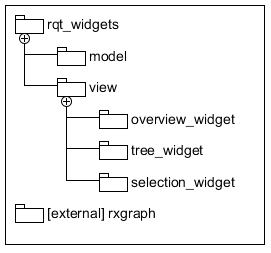
\includegraphics[scale=1.0]{./bilder/package_structure_gui.png}
\caption{The package structure of the GUI}
\label{The package structure of the GUI}
\end{center}
\end{figure}

\subsection{Model}

\begin{figure}[here]
\begin{center}
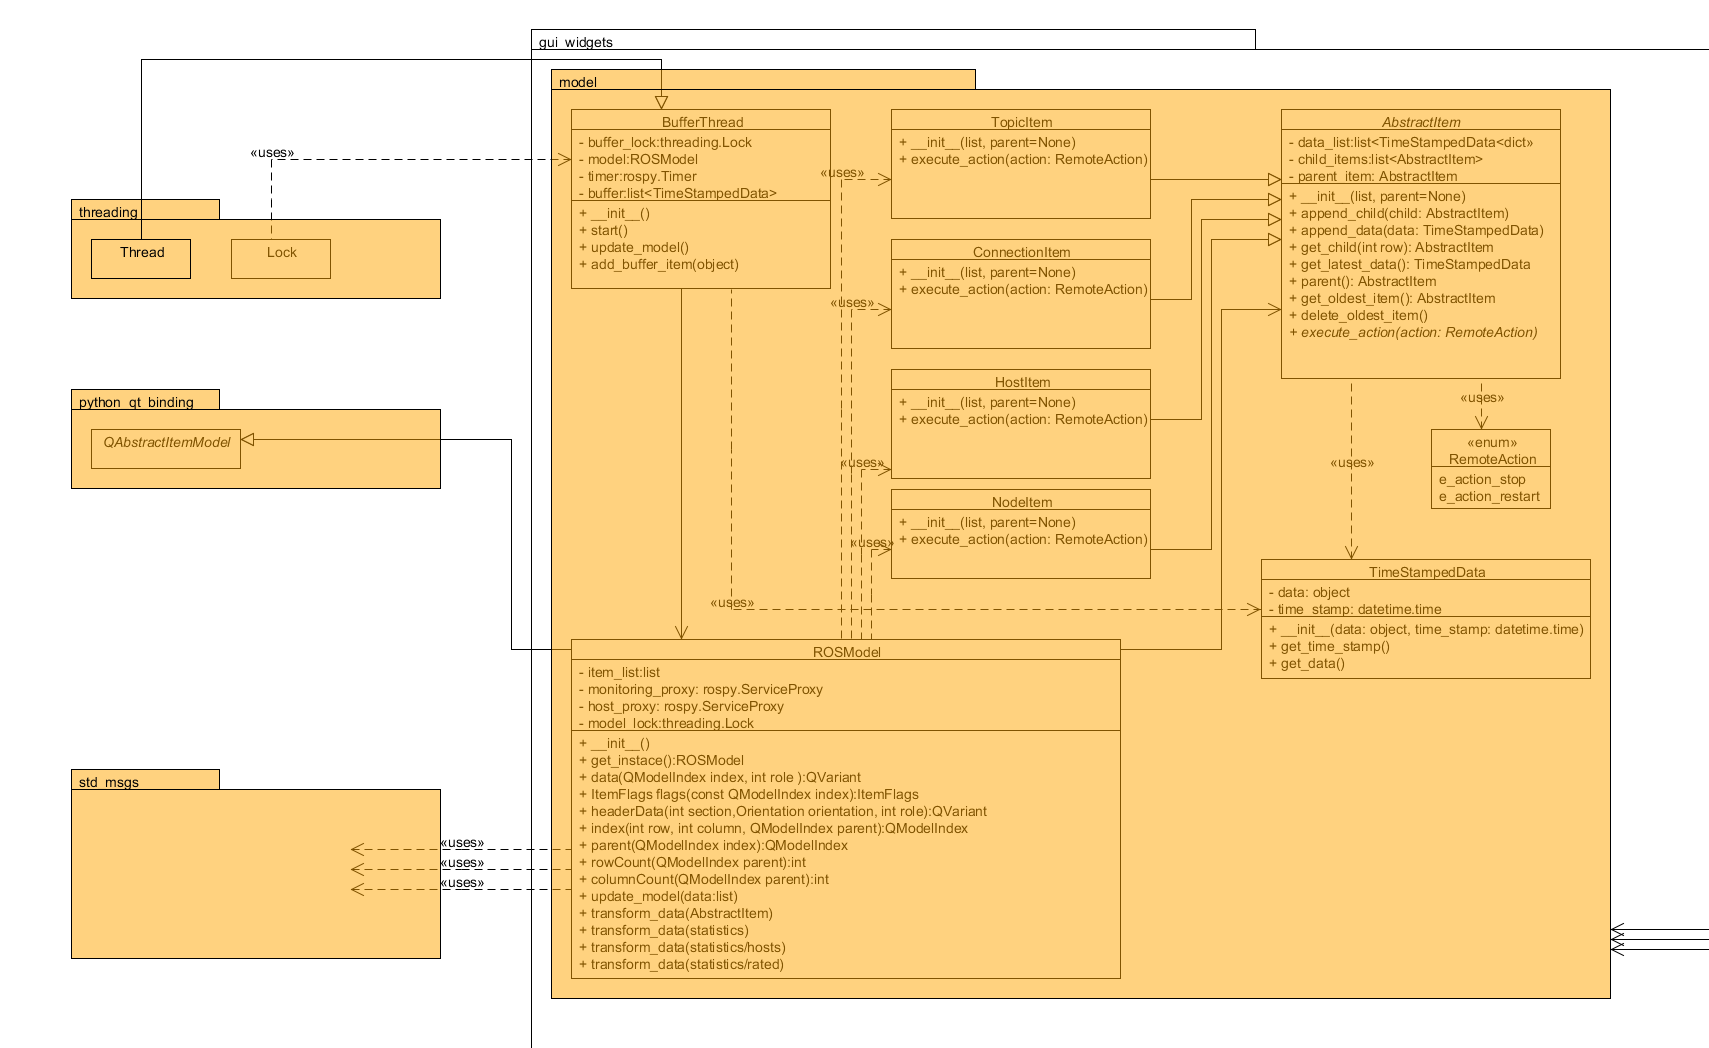
\includegraphics[width=1.0\linewidth]{./bilder/model.png}
\caption{The model class diagram}
\end{center}
\end{figure}

\subsubsection{BufferThread}
This thrad should buffer the incoming data and regulary update the model and hence also the model.
\subsubsection{ROSModel}
Represents the data as a QtModel. This enables automated updates of the View.
\subsubsection{ItemInterface}
Provides a unified interface to access the items of a model.
\subsubsection{HostItem}
A HostItem represents a host with all its data.
\subsubsection{NodeItem}
 A NodeItem represents a node with all of its data. It also has a interface to start/stop/restart nodes.

\subsection{View}

\begin{figure}[here]
\begin{center}
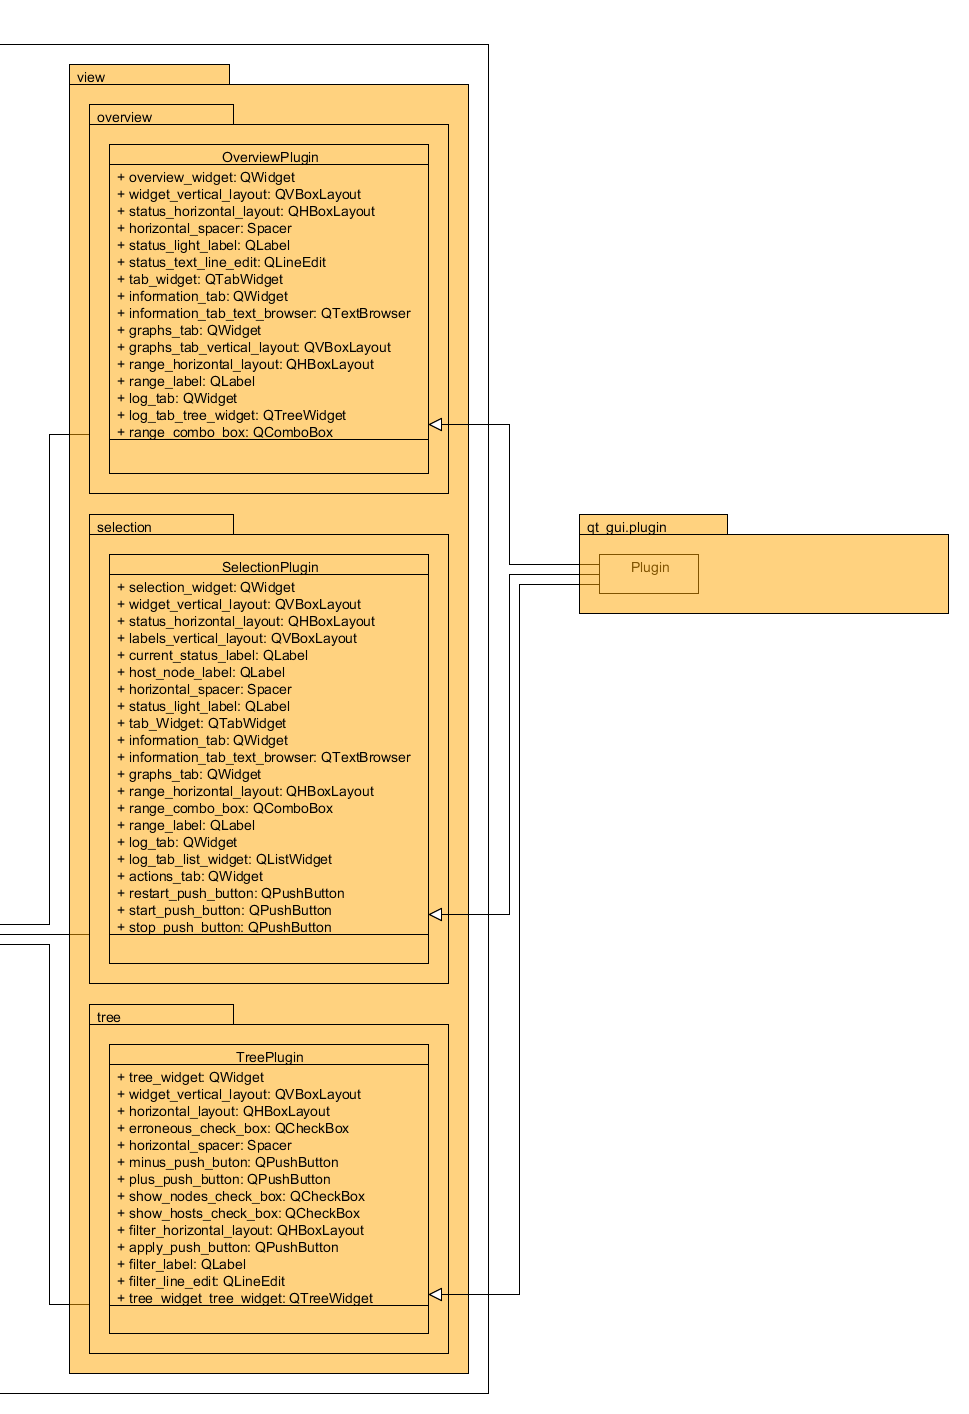
\includegraphics[width=\linewidth]{./bilder/view.png}
\caption{The view class diagram}
\end{center}
\end{figure}
\subsubsection{OverviewPlugin}
\subsubsection{TreePlugin}
\subsubsection{SelectionPlugin}